\begin{frame}
\frametitle{NEXT2-HD}

\begin{figure}[tbh!]
  \begin{center}
      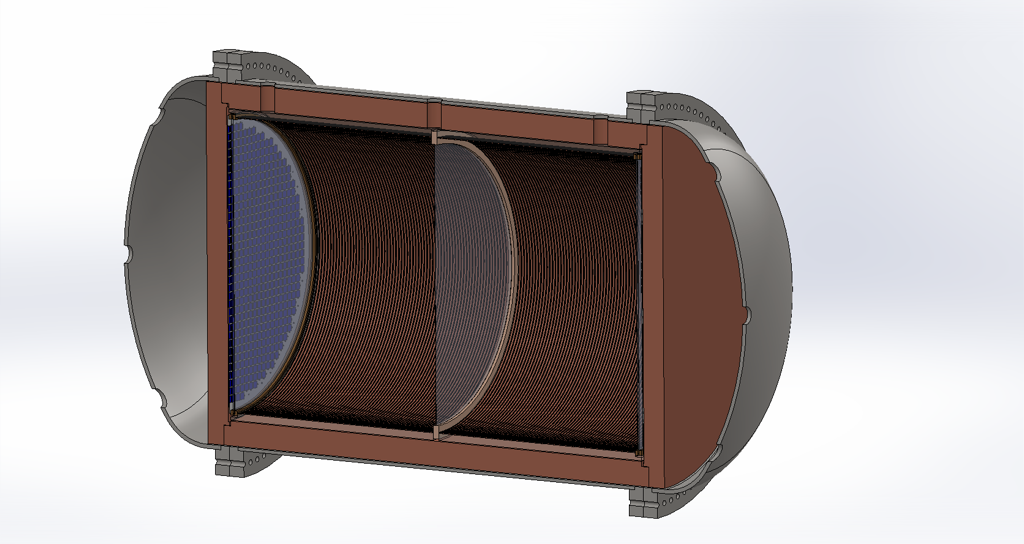
\includegraphics[width=0.75\textwidth]{moriond/next2.png}   
  \end{center}
\end{figure}

\begin{itemize}
\item Symmetric TPC: Diameter 2 m, drift length 3 m, pressure 20 bar, 1 ton per module.  
\item Uses only SiPMs mounted in ultra-pure substrates (gas cooled to -60 C).
  \item Low diffusion mixtures (Xe-He, Xe-CH$_4$). 
\end{itemize}
\end{frame}

\begin{frame}
\frametitle{NEXT2-HD improves rejection factor of topological signature}
\begin{figure}[tbh!]
  \begin{center}
      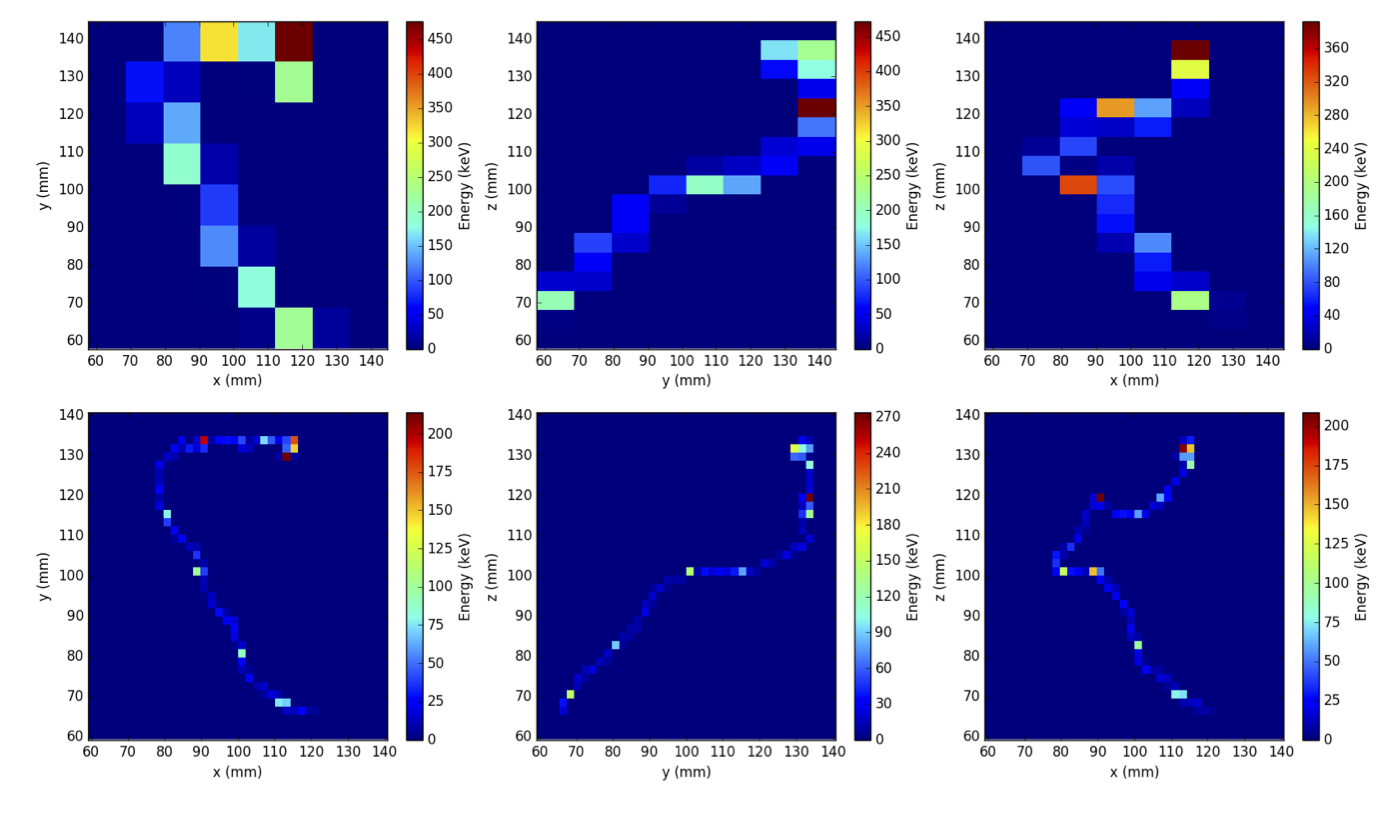
\includegraphics[width=0.45\textwidth]{moriond/high-low-diff-tracks.png}
       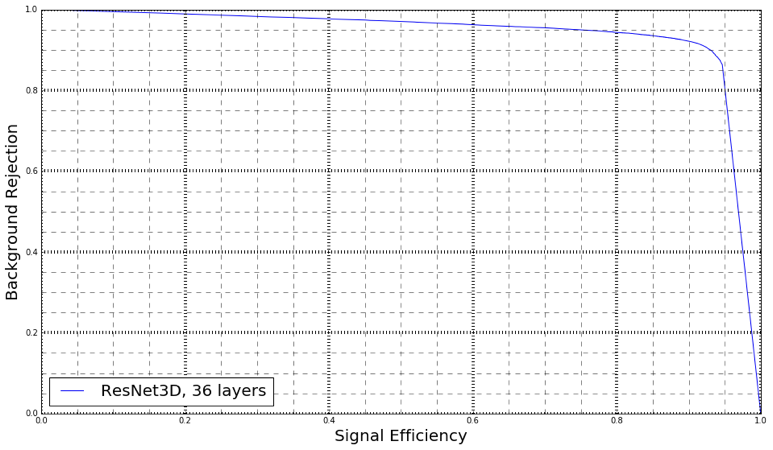
\includegraphics[width=0.45\textwidth]{moriond/signal-bkg-lowdiff-nn.png}
  \end{center}
 \end{figure}
 
 \begin{itemize}
\item Sharper topology results in an improvements of rejection factor by a factor 3.
\item Energy resolution may be further improved yielding a factor 2 (\BI\ peak very close to \Qbb).   
\end{itemize}
\end{frame} 

\begin{frame}
\frametitle{NEXT2-HD: incremental improvement approach}

\begin{columns}
 
\column{0.5\textwidth}
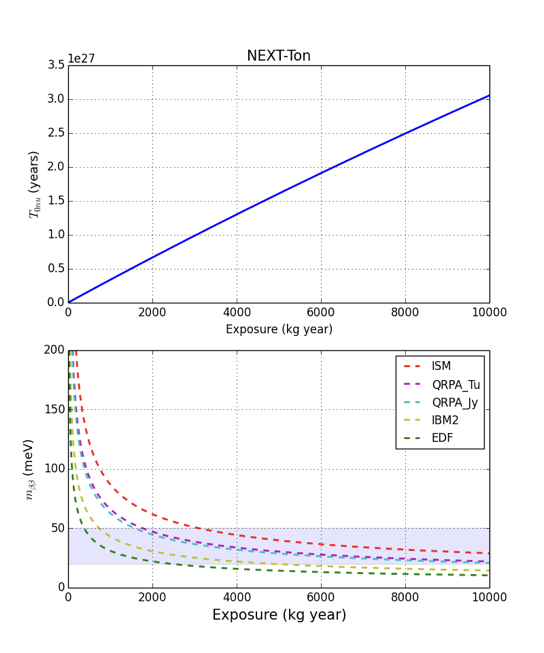
\includegraphics[scale=0.35]{moriond/next2-hd-sensi.png}
 
\column{0.5\textwidth}

%\begin{figure}[tbh!]
%  \begin{center}
%      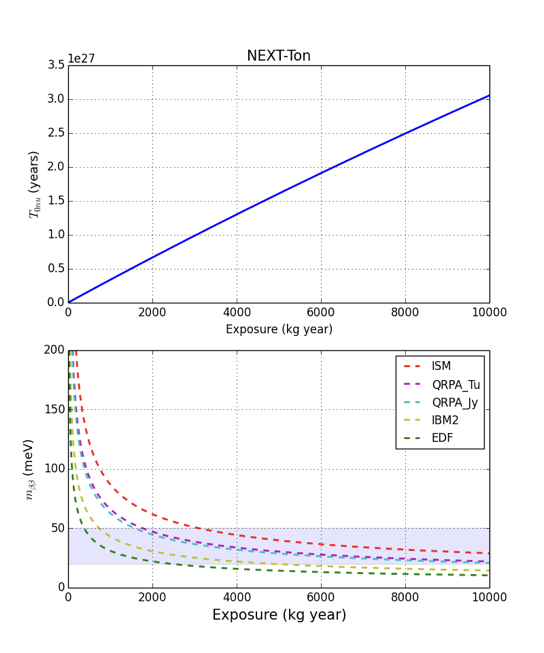
\includegraphics[width=0.4\textwidth]{moriond/next2-hd-sensi.png}
%   
%  \end{center}
% \end{figure}
 
\begin{itemize} 
\item SiPMs mounted in ultra-low background substrates, ultra-pure copper for inner shield, minimize materials inside TPC, deep underground location, water tank with neutron veto... an order of magnitude reduction in radioactive budget may be possible.   
\item Combination with improved topological signature and improved energy resolution may result in a ``background free'' detector at ton scale. 
\end{itemize}
\end{columns}
\end{frame}







